% !Mode:: "TeX:UTF-8"

\chapter{超像素分割和图像分割理论基础}

本文第1章介绍了超像素和图像分割的基本概念,并分类介绍了超像素分割和图像分割的研究背景及研究现状。
在本章中将对相关的基本理论进行简要的介绍。
首先简要叙述深度学习和神经网络的相关理论研究,接着介绍经典的基于神经网络的图像分割方法。
然后简述超像素在图像分割的意义。此外,介绍了将超像素整合到神经网络中的理论基础-超像素池化层。

\section{深度学习}
\begin{figure*}[h]
\begin{center}
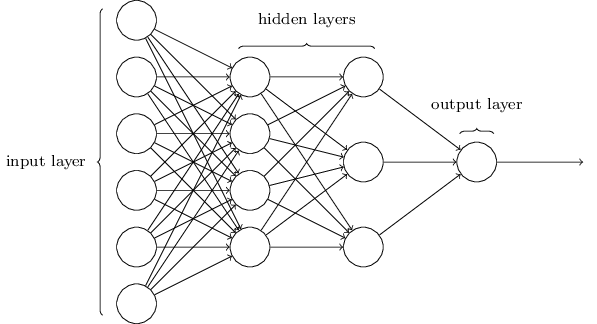
\includegraphics[width=1\textwidth]{figures/CNN0.png}
\end{center}
\vspace{-5mm}
\caption{多层感知器示意图}
\end{figure*}
%概念,分类,
2016年3月,在中央发表的"十三五"规划纲要中,“人工智能”一词格外引人注目。
BAT等各大互联网公司对人工智能领域的投入更是将人工智能这一领域的发展推向一个新的高潮。
目前深度学习无疑是人工智能的重点研究领域之一,设计到人工智能众多领域,如计算机视觉、自然语言处理等。

%浅层区别  《深度学习研究综述》
深度学习其实是机器学习的一种,从最初的浅层机器学习发展到目前深度学习。与浅层机器学习相比,深度学习加深了模型结构深度,一般有5 层,6 层,甚至更多的隐层节点。
一般而言,随着深度的增加,模型的学习能力也在增加。
此外,深度学习是一种特征学习,能够利用大数据来学习特征,从而能够获取数据更高层次的抽象表示,来描述数据的内在信息。

深度学习的概念源于人工神经网络的研究,深度学习网络最基本的结构是多层感知器(multilayer perception,MLP)。多层感知器,也就是我们所说的前向传播网络,一般有多层构成,每一层由若干神经元组成,如图2-1所示。



如图2-2所示,对于第$l$层,多层感知器的前向传播公式如下:
\begin{equation}
y_{i}^{k+1} = \sum_{j}W_{k}^{ij}y_{j}^{k}+b_{i}^{k}
\end{equation}
其中,$y_{j}^{k}$表示第k层的第j个神经元的输出,
$W_{k}^{ij}$表示第k层中第j个神经元与第k+1层的第i个神经元之间的权重,$b_{i}^{k}$是偏置值。
通常进行完这一步之后,会在此基础上使用非线性激活函数进行激活运算,常见的激活函数有ReLU、Sigmoid等。

\begin{figure*}[h]
\begin{center}
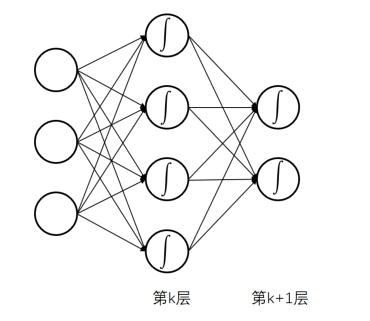
\includegraphics[width=1\textwidth]{figures/CNN01.png}
\end{center}
\vspace{-5mm}
\caption{前向传播示意图}
\end{figure*}
%应用
由于理论和计算力的原因,深度学习从提出到本世纪出,深度学习一度被边缘化,成果泛善可陈,直到2012年ImageNet比赛,多伦多大学团队开发的AlexNet模型的出现,以卷积神经网络( convolutional neural network)为基础,识别效果超过了所有浅层的方法。从此开启了深度学习进入快速发展的新时期,已经被广泛应用到计算机视觉、语言识别、自然语言处理等领域。

2015年的世界大规模人脸识别竞赛LFW中,来着香港中文大学多媒体实验室的中国团队使用深度学习模型,打败FaceBook 团队获得冠军。是的在人脸识别领域,深度学习的识别能力穿越真人。
此外在计算机视觉领域中的行人检测、多人姿态估计、物体跟踪、场景识别、图像分类、图像分割、物体跟踪等都有深度学习的身影。
近年来,科研人员也将深度学习应用到很多有意思的方向,例如:去除马赛克、风格迁移、黑白照片自动上色、图片补全等。

深度学习虽然很早应用于计算机视觉,在语音处理领域最先取得突破性进展。语音处理主要分为语音识别和语音合成两大方向。2016 年,微软利用深度学习开发的语言识别模型,在日常对话识别准确度上首先达到了人类水平,真正让大家大吃一惊。此外,各大公司也都在研究利用深度学习来进行语言合成,并已有成熟的系统,例如谷歌的WaveNet模型,百度的Deep Voice3。

2013年,Tomas Mikolov等人发表论文《Efficient Estimation of Word Representations in Vector Space》,提出了word2vector 模型,这也是目前自然语言处理通常使用的模型,与传统的词袋模型(bag of words)相比,word2vector能够更好地表达语法信息。
目前深度学习在自然语言处理领域的应用主要包括:问答系统、情感分析、机器翻译、句子成分分析等。
\section{卷积神经网络}

%定义
简单来说,卷积神经网络(Convolutional Neural Networks)是深度学习模型中的其中一类,类似于人工神经网络的多层感知器。
Yann LeCun在1994年提出的LeNet模型,最早将CNN应用于数字识别。2012年,多伦多大学Alex Krizhevsky等人开发的AlexNet模型第一次让大家注意到了CNN的强大之处。

% 网络结构
LeNet模型只有卷积层和池化层,全连接层,后来AlexNet模型在此基础上,加入了Relu激励层,提高了效率。接下来会分别介绍相关理论和计算。

\subsection{卷积层}
% 卷积操作
\begin{figure*}[h]
\begin{center}
%\fbox{\rule{0pt}{2in} \rule{.9\linewidth}{0pt}}
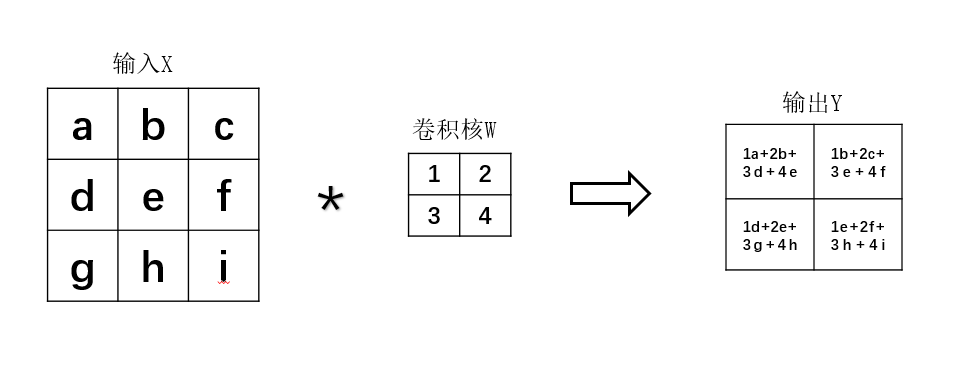
\includegraphics[width=1\textwidth]{figures/CNN1.png}
\end{center}
\vspace{-5mm}
\caption{卷积计算过程示意图}
\end{figure*}

卷积层作为卷积神经网络最重要的一层,其作用主要是提取图像的局部特征。如图2-2所示,卷积层的卷积操作为卷积核W与输入矩阵X 进行从左到右从上到下,步长为1的相乘相加操作,得出输出Y。卷积核W的大小为$M_w x N_w$,输入矩阵的大小为$M_x x N_x$,那么输出矩阵的大小等于$(M_x-M_w+1)x(N_x-N_w+1)$。
以图2-3为例,一个3x3的卷积核在一个5x5的输入图像上以步长为1做卷积计算,得到3x3的输出矩阵,这个输出矩阵就是特征矩阵。

\begin{figure*}[h]
\begin{center}
%\fbox{\rule{0pt}{2in} \rule{.9\linewidth}{0pt}}
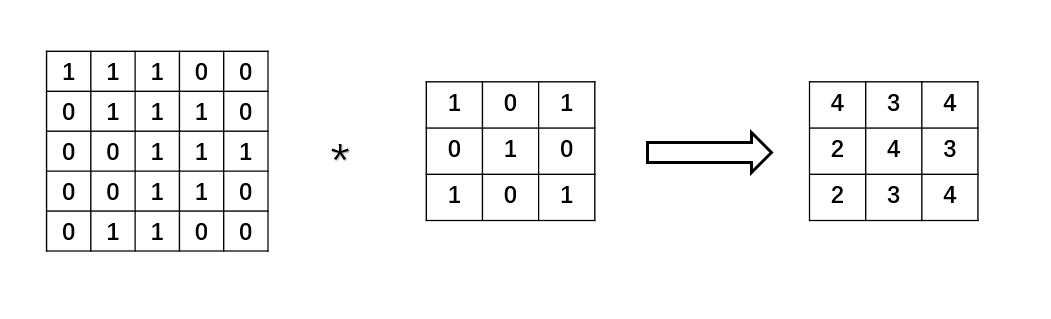
\includegraphics[width=1\textwidth]{figures/CNN2.png}
\end{center}
\vspace{-5mm}
\caption{卷积操作示意图}
\end{figure*}

\subsection{激活层}
%Relu激活
最原始的感知机(perceptron)并没有激活层,无论有多少层神经网络,输出层的结都是输入数据的线性组合,不能满足解决神经网络复杂任务的需求。因而加入了激活层,使用非线性函数作为激活函数,使得深层神经网络有了学习的能力,可以逼近任何函数。

用sigmoid函数和tanh函数作为最初的激活函数,输出有界,很容易充当下一层的输入。
随着神经网络的深度增加,卷积神经网络在反向传播过程中存在梯度消失的问题,
Sigmoid等激活函数的导数很小,而连续多个很小的数,结果几乎为0,因此梯度无法从输出层传到输入层。随着神经网络的深度增加会造成梯度消失的问题,从而导致训练难度大,效果不佳。此外,反向传播求梯度时,Sigmoid函数计算量较大。

2012年提出的AlexNet引入了一种新的激活函数-ReLU函数。该函数的提出很大程度的解决了BP算法在优化深层神经网络时的梯度耗散问题,而且减少了计算量。此外,Relu会使一部分神经元的输出为0,这样就造成了网络的稀疏性,并且减少了参数的相互依存关系,缓解了过拟合问题的发生。

现在也有一些对relu的改进,比如prelu,random relu等,对于不同的任务上,准确率或速度上有一定的改进。
此外,现在卷积神经网络,一般会在Relu激活层之后会多做一步归一化操作,尽可能保证每一层网络的输入具有相同的分布,减少计算量。

\subsection{池化层}
% 池化操作
在连续的卷积层之间一般会放入池化层,其目的是压缩数据,降低维度,减少计算。
池化层用的方法包括最大池化(Max pooling)和平均池化(Average pooling)。以最大池化为例,如图2-3所示,在一个4*4的矩阵上,选用2*2的filters,步长为2,对于每个2 * 2 的窗口选出最大的数作为输出矩阵的相应元素的值,比如输入矩阵第一个2 * 2窗口中最大的数是6,那么输出矩阵的第一个元素就是6,如此类推。平均池化的原理类似,只不过输出矩阵中的元素是输入矩阵对应窗口中元素的平均值。
\begin{figure*}[h]
\begin{center}
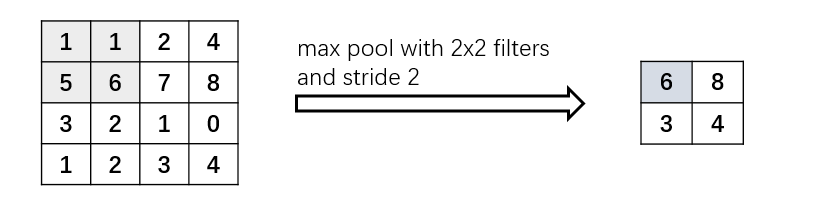
\includegraphics[width=1\textwidth]{figures/CNN3.png}
\end{center}
\vspace{-5mm}
\caption{池化操作示意图}
\end{figure*}

接下来具体介绍池化层的具体作用。如果输入数据是一张图片,那么池化层的作用就是对图像进行压缩。压缩过程中,去掉一些无关紧要的特征信息,留下最能体现图像特征的信息。我们知道,一张图像中含有的很多的信息,也具有很多的特征,但是有些特征信息,对于需要完成的任务则显得无关紧要,过于冗余。池化操作就是要去除这些冗余信息,留下最重要的特征信息。

池化操作具有特征不变性。所谓的特征不变性就是一张狗的图像被缩小了一倍,但还能认出这是一张狗的照片。
这说明在压缩过程中只是去除了无关紧要的信息,但对狗的重要特征信息仍有保留,因此我们依然可以能判断出这是一只狗。
% 发展
批归一化(Batch Normalization,BN)是深度学习发展中的一个里程碑式的技术,使各种网络能够进行训练。
在卷积神经网络训练过程中,由于参数是不断更新的,随着网络层数的加深,对于深层网络,其输入数值不稳定,导致模型很难收敛。通过归一化,对中间层的输出结果进行标准化处理,使得其更加稳定,分布更加固定,有利于算法的稳定和收敛。

然而,沿着批处理维度进行规范化会带来问题——当批处理大小变小时,BN的错误会迅速增加,这是由于批次统计估计不准确造成的。2018年,Yuxin Wu提出了Group Normalization,GN将通道分成组,并计算每组中的均值和方差进行归一化。GN的计算与批量大小无关,更适合于批次较小的任务。

\section{基于神经网络的图像分割}
《基于深度学习的RGB-D图像语义分割》
《FCN》http://www.sjocr.com/news/915.html
\section{超像素在图像分割中的意义}
%《基于图论的超像素分割及合并算法》
对于图像分割任务,基于像素的传统处理方法取得了不错的成果。
但是随着数码产品的拍照功能迅速发展,图像的构成越来越复杂,分辨率不断增大,越来越清晰,包括的像素数量也是成指数级增长。
在这样的背景下,基于像素的传统图像分割方法处理分辨率高的图像,将花费更多的时间。

如何减少图像分割的计算量显得尤为重要。超像素作为一种图像预处理技术解决了这个问题。
所谓超像素,就是由局部的许多像素构成的区域,这些区域内的像素通常由具有相似纹理、颜色、亮度等特征。
相对于像素而言,超像素不仅有效减少了局部的冗余信息,后续处理过程中的计算量和复杂度大幅度降低,而且更利于局部特征的提取与表达,更有利于帮助定位区域的边界。

\section{超像素池化层}

2017年,Suha Kwak等人提出了Superpixel Pooling Network (SPN)网络,将超像素分割结果作为低阶结构的表征,利用提出的超像素池化层对输入网络的超像素进行提取特征,辅助语义分割的推断。
此外,SPN网络验证了使用了Superpixel可以提高图像分割的准确率,确实能起到一定的效果。

在这里简单介绍一下SPN网络中超像素池化层的具体操作,每个超像素的特征向量生成如公式2-2所示:
假设 $P_{i}= \left \{ p_{i}^{k} \right \} k=1,2,\cdots ,K_i$ 表示图像中第i个Superpixel,$K_i$表示第i个Superpixel 中像素的个数,对于每个Superpixel i,feature vector 的生成公式:

\begin{equation}
v_{i} = \frac{1}{K_i}\sum_{j}\sum_{k}I(p_{i}^{k}\in r^{j})z^{j}
\end{equation}
其中,$r^{j}$表示感受野, $z^{j}$表示经过上采样得到的特征图中的第j个位置的值。 $I(p_{i}^{k}\in r^{j})$是一个indicator 函数,如果括号中的值为true,则返回1,否则返回0。

固定当前某一个超像素,将之池化。式中的$r$存在是因为存在尺度差异,是感受野大小。
作者的池化方式是固定超像素,遍历特征图和超像素内的元素,计算当前超像素元素在位置j感受野所占的比例,然后加权上去。
通过式2-2便可以得到每个超像素的特征向量,从而可进行后续的运算。
